\documentclass{article}

\usepackage[utf8]{inputenc} % obsługa UTF-8
\usepackage[T1]{fontenc} 	% kodowanie fontów
\usepackage[polish]{babel} 	% pakiet dla języka polskiego
\usepackage[ruled,vlined]{algorithm2e}
\usepackage{geometry} % ustawienia marginesów	
\usepackage{graphicx} % wstawianie grafiki
\usepackage{caption} 	% wstawianie podpisów
\usepackage{amsmath} % wprowadzanie wzorów
\usepackage{float}
\usepackage{textgreek} % obsługa znaków greckich
\usepackage{booktabs}
\usepackage{tabularx} % Lepsza obsługa tabel

\geometry{	
	 	 a4paper, % Rozmiar papieru	
	 	 left=15mm, % Lewy margines	
	 	 right=15mm, % Prawy margines	
	 	 top=25mm, % Górny margines	
	 	 bottom=25mm, % Dolny margines	
	 	}
\geometry{columnsep=1cm}

\makeatletter
\newcommand{\linia}{\rule{\linewidth}{0.4mm}}
\renewcommand{\maketitle}{\begin{titlepage}
	 	 \vspace*{1cm}
	 	 \begin{center}\small
	 	 Politechnika Rzeszowska\\
	 	 Wydział Matematyki i Fizyki Stosowanej\\
	 	 \end{center}
	 	 \vspace{3cm}
	 	 \begin{center}
	 	 	\scalebox{4}{Sprawozdanie}
            \begin{center}\Large
                Alorytmy i struktury danych
            \end{center}
	 	 \end{center}
	 	 \noindent\linia
	 	 \begin{center}
	 	 	 \LARGE \textsc{\@title}
	 	 	 	 	\end{center}
	 	 	\linia
	 	 \vspace{0.5cm}
	 	 \begin{flushright}
	 	 \begin{minipage}{30cm}
	 	 \textit{\small Autor:}\\
	 	 \normalsize \textsc{\@author} \par
	 	 \end{minipage}
	 	 \vspace{5cm}
	 	 	\end{flushright}
	 	 \vspace*{\stretch{6}}
	 	 \begin{center}
	 	 \@date
	 	 \end{center}
	 \end{titlepage}
}
\makeatother
\author{Mateusz Działowski}
\title{Zadanie projektowe/algorytmiczne}
\date{20 stycznia 2026}
\begin{document}

\maketitle

\newpage
\tableofcontents
\renewcommand{\figurename}{Rys.} 
\newpage
\section{Wstęp}
Celem niniejszego opracowania projektu jest przedstawienie implementacji oraz analizy wydajnościowej algorytmu, rozwiązującego problem wyszukiwania specyficznych podciągów w zadanym ciągu liczb całkowitych dodatnich wejściowych. Dokumentacja obejmuje szczegółowy opis problemu, podstawy teoretyczne, implementację algorytmu oraz wyniki testów wydajnościowych przeprowadzonych na różnych zestawach danych wejściowych.

\vspace{0.4cm}

"W przedstawionym opracowaniu indexowanie pozycji w podciagach i tablicach zaczyna się od 0."

\vspace{0.4cm}

\newpage
\section{Opis problemu}

Dla zadanego ciagu liczby całkowitych dodatnich ciagu A$[]$ o długości N, należy znaleźć wszystkie podciagi o długości M = 5 (pięcioelementowe) w danym ciagu, które spełniają kryterium: Suma elementów na pozycji 2 i 4 jest wieksza od sumy elementów na pozycji 1, 3 i 5.

Dla, podciagu T$[]$ = $[t_0,t_1,t_2,t_3,t_4]$, warunek przyjmuje postać:

\vspace{0.6cm}

\begin{equation}
    t_1 + t_3 > t_0 + t_2 + t_4
\end{equation}

\vspace{0.6cm}

{\bfseries Przykład:} Dla ciagu A$[]$ = $[1, 130, 1, 9, 11, 6, 1, 1, 1, 3, 1]$, zgodnie z powyższym kryterium, podciagi spełniające warunek to:

\begin{itemize}
	\item T$[M]$ = $[1, 130, 1, 9, 11]$, ponieważ (130 + 9 > 1 + 1 + 11)
	\item T$[M]$ = $[1, 9, 11, 6, 1]$, ponieważ (9 + 6 > 1 + 11 + 1)
	\item T$[M]$ = $[1, 1, 3, 1, 1]$, ponieważ (1 + 1 > 1 + 3 + 1)
\end{itemize}

Jak widać, w powyższym przykładzie istnieją trzy podciagi spełniające zadane kryterium.

\section{Podstawy teoretyczne}

Algorytmy opiera sie na technice przesuwania okna o stałej M = 5. Dla kazdego możliwego podciagu o długości M w ciągu A$[]$, algorytm sprawdza, czy spełnia on warunek określony w równaniu (1). Jeśli tak, podciag jest zapisywany do wyniku.
\subsection{Złożoność algorytmu}
Teoretyczna analiza złożoności algorytmu przedstawia się następująco:
\begin{itemize}
    \item {\bfseries Złożoność czasowa:} Sprawdzenie jednego okna zajmuje czas stały $O(1)$. Ponieważ okno przesuwamy przez cały ciąg o długości $N$, wykonujemy $N-M+1$ operacji, M jest stałą co powoduje że teoretyczna złożoność powinna wynosić $O(N)$.
    \item {\bfseries Złożoność obliczeniowa:} Algorytm wymaga przechowywania ciągu wejściowego o wielkości N oraz tablicy wyników M, która jest stałą. Rówanie wyglada następująco: $O(N+M)$, co teoretyczne w najgorszym przypadku, gdy każdy podciąg spełnia warunek złożoność pamięciowa wynosi $O(N)$.
\end{itemize}

\section{Szczegóły implementacji}
\subsection{Rozwiazanie problemu - podejście pierwsze}
\subsubsection{Analiza problemu}

Choć algorytm jest stosunkowo prosty, jego implementacja wymaga uwzględnienia kilku kluczowych aspektów, takich jak efektywne zarządzanie pamięcią, optymalne podejście przy wykorzystaniu pętli oraz optymalizacja operacji sprawdzania warunków, co może znacząco wpłynąć na wydajność końcowego rozwiązania. Pod uwage trzeba wziąść również obsługę różnych przypadków brzegowych, takich jak bardzo krótkie ciągi wejściowe lub ciągi nie spełniające żadnego z kryteriów co wciąż wpływa na wydajność implementacji.

\vspace{0.2cm}
W podejściu pierwszym, postąpimy w sposób bezpośredni, iterując przez każdy możliwy podciąg o długości M w ciągu A$[N]$ i sprawdzając, czy spełnia on warunek określony w równaniu (1). Jeśli tak, dodajemy go do listy wyników, liście wyników nie przypisujemy żadnej wartości elementowej ponieważ przyjmujemy, że tablica dynamicznie zmienia swoje rozmiary.
Również musimy wziąść pod uwagę przypadki, gdy długość ciągu N jest mniejsza niż M lub dane wejściowe są ułożone w sposób uniemożliwiający znalezienie podciągu spełniającego warunek. W takim przypadku nie ma możliwości znalezienia żadnego podciągu o wymaganej długości, więc algorytm powinien zwrócić pustą listę wyników.

\vspace{0.4cm}
1. Dane wejściowe.\\
\hspace*{1cm} Naszymi danymi wejściowymi są: 
\begin{itemize}
	\setlength{\leftskip}{1cm}
	\item Ciąg liczb całkowitych dodatnich Tab$[]$ również,
	\item długość ciągu N,
	\item stała M = 5.
\end{itemize}

	2. Dane wyjściowe.\\
\hspace*{1cm} Naszymi danymi wyjściowymi są: 
\begin{itemize}
	\setlength{\leftskip}{1cm}
	\item Tablica wyników Wynik$[]$, zawierająca wszystkie podciągi.
\end{itemize}

\vspace{0.4cm}

Implementacja wykorzystuje zagnieżdżone pętle iteracyjne (warunki zapętlone), wraz z zmiennym sterującymi, aby efektywnie przeszukiwać ciąg wejściowy i identyfikować podciągi spełniające określone kryteria. Poniżej przedstawiono szczegółowy opis działania poszczególnych pętli:

\begin{itemize}
    \item {\bfseries Pętla zewnętrzna i < N-4 (\texttt{i})} - przesuwa okno przez cały ciąg (od 0 do N-4), że względu na warunek sprawdzający (1) musimy pętle ograniczyć do N-4, w celu uniknięcia błędów. Przedstawionej pętli sprawdzamy krok po kroku każdy możliwy podciąg o długości M = 5, czy spełnia on warunek z równania (1), również pętla przesuwa okno o jeden element do przodu w każdej iteracji w celu sprawdzenia następnych możliwych podciągów.
    \item {\bfseries Pętla wewnętrzna j < N-4 (\texttt{j})} - rozpoczyna się od pozycji {\bfseries j = i} i iteruje do N-4, sprawdzając warunek z równania (1) dla każdego podciągu zaczynającego się na pozycji \texttt{i}.
    \item {\bfseries Pętla iteracyjna k < M (\texttt{k})} - przechodzi przez elementy podciągu (od 0 do M-1), aby obliczyć sumy wymagane do sprawdzenia warunku z równania (1). W tej pętli sumujemy odpowiednie elementy podciągu, aby porównać je zgodnie z kryterium określonym w równaniu (1).
    \item {\bfseries Pętla kopiująca m < M (\texttt{m})} - przepisuje spełniający warunek podciąg do tablicy wyników Wynik$[]$. Ta pętla iteruje przez elementy podciągu i kopiuje je do tablicy wyników, gdy warunek z równania (1) jest spełniony.
\end{itemize}

Gdy warunek z równania (1) zostanie spełniony dla danego okna, algorytm kopiuje 5 elementów do tablicy wyników i przerywa wewnętrzne pętle poprzez ustawienie wartości sterujących (\texttt{j = N}, \texttt{k = M}), co wymusza przejście do następnej pozycji okna.
\newpage
\subsubsection{Schemat blokowy algorytmu}
Poniżej przedstawiono schemat blokowy ilustrujący działanie algorytmu:



\begin{figure}[H]
	\centering
	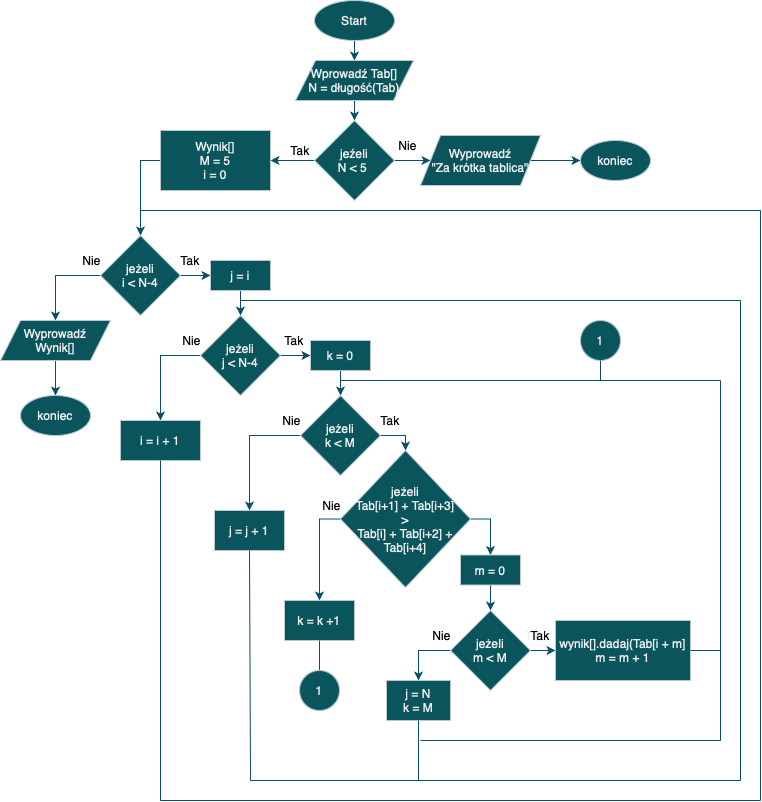
\includegraphics[width=0.9\linewidth]{../Dane/Diagram_1.png}
	\caption{Schemat blokowy algorytmu wyszukiwania podciągów}
	\label{fig:diagram}
\end{figure}

\newpage

\subsubsection{Algorytm zapisywany w pseudokodzie}
W poniższym pseudokodzie przedstawiono szczegółową implementację algorytmu. W przypadku pseudokodu, przyjeliśmy wykorzystanie pętli while do iteracji przez elementy ciągu oraz do sprawdzania warunków w porównaniu do schematu blokowego gdzie przyjeśliśmy warunki jako pętle.\\
W pseudokodzie użyto następujących oznaczeń:
\begin{itemize}
	\item \texttt{Tab[]} - tablica wejściowa zawierająca ciąg liczb całkowitych dodatnich,
	\item \texttt{N} - długość tablicy wejściowej,
	\item \texttt{wynik[]} - tablica wynikowa przechowująca znalezione podciągi,
	\item \texttt{M} - stała określająca długość podciągu (M = 5),
	\item \texttt{i, j, k, m} - zmienne sterujące pętli.
\end{itemize}

\begin{algorithm}[H]
\SetKwInOut{Input}{Input}\SetKwInOut{Output}{Output}
\Input{Tab[], N}
\Output{wynik[] lub $-1$}
\If{$N < 5$}{\Return $-1$}
wynik $\gets$ [ ]\;
\SetKw{KwConst}{const}
\KwConst $M \gets 5$\;
i $\gets$ 0\;
\While{$i < N - 4$}{
  j $\gets$ i\;
  \While{$j < N - 4$}{
    k $\gets$ 0\;
    \While{$k < M$}{
      \If{$Tab[i+1] + Tab[i+3] > Tab[i] + Tab[i+2] + Tab[i+4]$}{
        m $\gets$ 0\;
        \While{$m < M$}{
          wynik.\texttt{dodaj}$(Tab[i + m])$\;
          m $\gets$ m + 1\;
        }
        j $\gets$ N\;
        k $\gets$ M\;
      }
      \Else{
        k $\gets$ k + 1\;
      }
    }
    j $\gets$ j + 1\;
  }
  i $\gets$ i + 1\;
}
\Return wynik\;
\end{algorithm}

Jak widać, algorytm iteruje przez każdy możliwy podciąg o długości M w ciągu Tab$[]$, sprawdzając, czy spełnia on warunek określony w równaniu (1). Jeśli tak, podciąg jest dodawany do tablicy wyników wynik$[]$. W przypadku, gdy długość ciągu N jest mniejsza niż M, algorytm zwraca $-1$, wskazując na brak możliwości znalezienia podciągu spełniającego warunek.
\newpage
\section{Sprawozdanie poprawności algorytmu}
Aby zweryfikować poprawność działania zaimplementowanego algorytmu, przedewszystkim przeprowadzimy test "ołówkowy" 
\end{document}